\chapter{Tinjauan Pustaka dan Dasar Teori}

Bab ini menuliskan teori dan konsep yang melandasi penelitian berdasar acuan primer (Riset dalam jurnal ilmiah) yang up to date dan relevan. Uraikan dengan jelas kajian pustaka 
(dari referensi) yang menimbulkan gagasan dan mendasari kegiatan Skripsi sesuai tema atau judul yang diambil. Sumber-sumber yang cocok untuk tinjauan pustaka meliputi:

\begin{enumerate}
\item Buku-buku, monograf, buletin, laporan, dan artikel penelitian tertentu – maksimal 
penelitian atau tulisan dalam 10 tahun terakhir, semakin baru semakin bagus.
\item Materi yang tidak dipublikasikan (misalnya, disertasi, tesis, makalah yang 
dipresentasikan pada pertemuan profesional baru-baru ini yang belum dipublikasikan, 
dll.)
\end{enumerate}

\noindent Secara umum bab ini berisi informasi tentang:

\begin{enumerate}
\item Latar belakang dan tujuan dari penelitian
\item Definisi dan konsep-konsep yang relevan dalam bidang tersebut
\item Studi kasus atau penelitian terdahulu yang terkait dengan masalah yang diteliti
\item Analisis dan kritik terhadap penelitian sebelumnya
\item Kerangka teori dan hipotesis dasar
\item Metodologi yang akan digunakan dalam penelitian
\item Batasan dan kerangka waktu penelitian.
\end{enumerate}

\section{Latar Belakang Masalah}

Berikut ini adalah contoh tinjauan pustaka perancangan rangkaian penguat audio. Rangkaian penguat audio adalah sistem yang memperkuat sinyal audio masukan menjadi sinyal 
audio yang lebih kuat. Rangkaian penguat audio memiliki banyak aplikasi dalam bidang audio, seperti sistem home theater, sistem pemutar musik, dan lain-lain. Tujuan dari tinjauan pustaka ini adalah untuk meninjau dan menganalisis
berbagai jenis rangkaian penguat audio dan teknik-teknik
yang digunakan dalam perancangan rangkaian penguat audio. Selanjutnya dapat diuraikan di sub-bab selanjutnya atau bab \ref{ch2-definisi-dan-konsep-dasar}. 


\section{Definisi dan Konsep Dasar}
\label{ch2-definisi-dan-konsep-dasar}

Pertama, definisi dan konsep dasar dari rangkaian penguat audio akan dibahas di sini. Konsep-konsep ini meliputi pengertian sinyal audio, karakteristik sinyal audio, dan jenis-jenis rangkaian penguat audio.

\section{Studi Kasus atau Penelitian Terdahulu}

Di sini akan membahas berbagai studi kasus atau penelitian terdahulu yang berhubungan dengan perancangan rangkaian penguat audio. Teknik-teknik yang digunakan 
dalam perancangan rangkaian penguat audio, kinerja dan efisiensi dari rangkaian penguat audio, dan perbandingan antar jenis rangkaian penguat audio yang berhubungan dengan 
penyelesaian masalah akan dibahas secara detail.


\section{Analisis dan kritik terhadap penelitian sebelumnya}

Di sini akan dilakukan analisis dan kritik terhadap penelitian sebelumnya untuk menentukan kelemahan dan kelebihan dari masing-masing teknik perancangan rangkaian 
penguat audio yang pernah ada.


\section{Kerangka Teori dan Hipotesis Dasar}

Di sini akan disusun kerangka teori dan hipotesis dasar yang akan digunakan sebagai dasar dalam perancangan rangkaian penguat audio. Seperti misalnya, Penguat kelas D yang 
akan digunakan, adalah yang paling bagus efisiensinya, dipilih dari yang sudah dibahas pada sub-bab sebelumnya, yaitu analisis dan kritik penelitian terdahulu, atau hasil gabungan dari beberapa teori atau hasil penelitian sebelumnya.

\section{Metodologi yang Akan Digunakan}

Di sini akan dibahas metodologi yang akan digunakan dalam perancangan rangkaian penguat audio, termasuk jenis-jenis peralatan yang akan digunakan, teknik-teknik yang akan 
digunakan untuk menguji kinerja dan efisiensi rangkaian penguat audio, dan prosedur yang akan digunakan untuk memperoleh hasil yang akurat. Sub bab ini ringkasan saja, detailnya akan dibahas di Bab Metode Penelitian.

\section{Batasan dan Kerangka Waktu Penelitian}

Terakhir, kita akan membahas batasan dan kerangka waktu penelitian, termasuk batasan sumber daya yang tersedia dan berapa lama waktu yang tersedia untuk menyelesaikan 
penelitian ini.

\section{Dasar Teori}

Setelah metodologi ditentukan, maka akan ada tentang teknik-teknik, sistem, teknologi atau komponen-komponen yang digunakan. Hal-hal tersebut dapat dituliskan di sub bab Dasar 
teori ini. Dasar teori pada umumnya diperoleh melalui buku referensi, publikasi tugas akhir, dan informasi web yang dapat dipertanggungjawabkan. Hindari penggunaan dasar teori 
melalui tautan wikipedia, surat kabar, atau portal berita.

\vspace{1cm}

\noindent\textbf{Contoh Penulisan Dasar Teori: Pengenalan Aplikasi Permainan}

Proses pembuatan \textit{game} dimulai dari pembuatan \textit{game design document} dimana 
dokumen ini akan menjadi landasan pengembangan game tersebut serta menginformasikan gambaran keseluruhan game yang akan dibuat \cite{ferdiana2012agile}. \textcolor{red}{\textit{Catatan: apapun yang diambil dari tulisan orang lain harus disitasi seperti dicontohkan \cite{ferdiana2012agile}.}}

\begin{figure}[h]
	\centering
	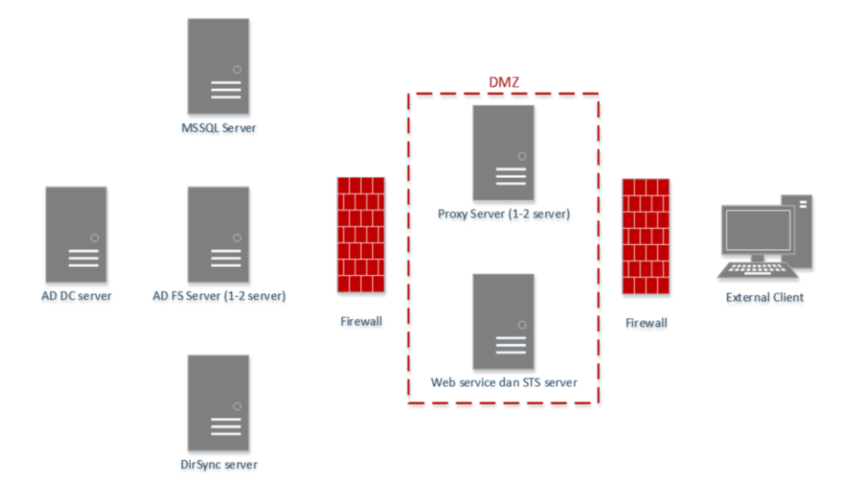
\includegraphics[width=12cm]{contents/chapter-2/gambar-buatan-sendiri.png}
	\caption{Contoh gambar}
	\label{Fig:gambar-buatan-sendiri}
\end{figure}

\textit{Game design document} adalah sebuah bagian penting dalam pembuatan game baik itu elemen-elemen penyusunnya maupun proses pengembangannya. Game design yang telah dibuat, dijabarkan satu persatu mengenai tahapan dalam pembuatan game dan hasilnya disatukan dalam bentuk dokumentasi \textit{game design document} yang digunakan oleh \textit{developer} sebagai buku petunjuk bagaimana membuat \textit{game} \cite{lukito2016}.

Dalam buku \textit{Game Design Essentials} disebutkan \textit{game design document} merupakan metode yang menghubungkan elemen-elemen penyusun \textit{game}, baik itu \textit{art, sound, program, 
gameplay} sehingga semuanya terdokumentasi menjadi satu dan menjadi acuan bagi para \textit{developer} dalam membuat \textit{game} \cite{wibirama2013dual}. 
